% ═══════════════════════════ ANEXOS ═══════════════════════════
\clearpage
\appendix
\renewcommand{\thesection}{\Alph{section}}
\addtocontents{toc}{\protect\renewcommand{\protect\cftsecnumwidth}{4.6em}}
\renewcommand{\cftsecpresnum}{Anexo~}
\titleformat{\section}
  {\large\bfseries}
  {Anexo~\thesection\ \hspace{0.4em}}{0em}
  {}[\vspace{2pt}{\color{rule}\titlerule[0.4pt]}]
\setcounter{section}{0}

% ───────────────────────────────────────────────
\section{Diagrama de arquitectura de eventos}
\label{anx:arq}

La Figura~\ref{anx:diag} muestra el flujo completo. Una sola publicación al exchange se reparte en fan-out a dos colas. El Scoring Worker encadena un segundo evento que activa al Ranking Worker. El evento \code{round.closed} llega por el administrador o por el scheduler automático.

\vspace{6pt}
\begin{figure}[h]
\centering
\resizebox{\linewidth}{!}{%
\begin{tikzpicture}[
  font=\footnotesize,
  box/.style={rectangle,draw=ink!35,fill=white,
              align=center,minimum height=0.9cm,minimum width=2.4cm,inner sep=4pt},
  exch/.style={rectangle,draw=ink,line width=0.6pt,fill=ink!4,
               align=center,minimum height=1.0cm,minimum width=2.7cm,inner sep=4pt},
  queue/.style={cylinder,shape border rotate=90,draw=ink!45,fill=white,
                minimum height=0.55cm,minimum width=1.95cm,inner sep=2pt,aspect=0.32,
                font=\scriptsize\ttfamily,align=center},
  worker/.style={rectangle,draw=ink!55,fill=ink!3,
                 align=center,minimum height=0.9cm,minimum width=2.3cm,inner sep=4pt},
  db/.style={cylinder,shape border rotate=90,draw=ink!45,fill=white,
             minimum height=0.7cm,minimum width=2.0cm,inner sep=3pt,aspect=0.28,
             font=\scriptsize,align=center},
  arr/.style={-{Stealth[length=2.2mm]},semithick,color=ink!55},
  arrd/.style={-{Stealth[length=2.2mm]},semithick,dashed,color=ink!70},
  arrg/.style={-{Stealth[length=1.8mm]},thin,color=muted},
  lbl/.style={font=\scriptsize\ttfamily,color=muted,inner sep=1.5pt},
  lblo/.style={font=\scriptsize\ttfamily,color=ink,inner sep=1.5pt}
]

\node[box] (api) {Backend API\\[1pt]\scriptsize\rmfamily FastAPI};
\node[box,below=1.7cm of api] (sched)
      {Scheduler\\[1pt]\scriptsize\rmfamily cada 60 s};

\node[exch,right=3.4cm of api,yshift=-0.85cm] (exch)
      {\rmfamily Exchange\\[1pt]\scriptsize\ttfamily pickandserve.events\\[1pt]\scriptsize\rmfamily(topic)};
\node[lblo] at ([yshift=0.42cm,xshift=0.2cm]exch.north) {fan-out};

\node[queue,right=2.5cm of exch,yshift=2.55cm]  (q1) {scoring.queue};
\node[queue,below=0.5cm of q1]                  (q2) {notifications\\.queue};
\node[queue,below=0.5cm of q2]                  (q3) {ranking.queue};
\node[queue,below=0.5cm of q3]                  (q4) {notifications\\.round.queue};

\node[worker,right=1.5cm of q1] (w1) {Scoring\\[1pt]Worker};
\node[worker,right=1.5cm of q2] (w2) {Notification\\[1pt]Worker};
\node[worker,right=1.5cm of q3] (w3) {Ranking\\[1pt]Worker};

\node[db,below=0.75cm of q4,xshift=1.4cm] (db) {\rmfamily PostgreSQL};

\draw[arr] (api.east) -- (exch.west);
\node[lbl,above,yshift=1pt] at ($(api.east)!0.5!(exch.west)$) {\scriptsize match.result.loaded};

\draw[arr] (exch.east) -- (q1.west);
\draw[arr] (exch.east) -- (q2.west);
\draw[arr] (exch.east) -- (q3.west);
\draw[arr] (exch.east) -- (q4.west);

\draw[arr] (q1) -- (w1);
\draw[arr] (q2) -- (w2);
\draw[arr] (q3) -- (w3);
\draw[arr] (q4.east) -| (w2.south);

\draw[arrd] (w1.north) -- ++(0,0.45) -| node[lblo,pos=0.25,above]{scores.updated} ($(q3.north)+(-0.15,0)$);

\draw[arr] (sched.east) -| node[lbl,pos=0.25,below]{round.closed} ($(exch.south)+(0,0)$);

\draw[arrg] (w1.east) -- ++(0.35,0) |- (db.east);
\draw[arrg] (w2.east) -- ++(0.55,0) |- (db.east);
\draw[arrg] (w3.east) -- ++(0.35,0) |- (db.east);

\end{tikzpicture}}
\caption{Flujo de eventos de Pick \& Serve. El trazo continuo muestra el enrutamiento del broker, el punteado el encadenamiento de eventos, y el gris la persistencia en la base de datos.}
\label{anx:diag}
\end{figure}

\vspace{2pt}
\begin{center}
\small
\begin{tabularx}{0.92\linewidth}{@{}>{\ttfamily}l >{\ttfamily}l X@{}}
\toprule
\textbf{Cola} & \textbf{Routing key} & \textbf{Worker} \\
\midrule
scoring.queue & match.result.loaded & Scoring Worker \\
notifications.queue & match.result.loaded & Notification Worker \\
ranking.queue & scores.updated & Ranking Worker \\
notifications.round.queue & round.closed & Notification Worker \\
\bottomrule
\end{tabularx}
\end{center}

% ───────────────────────────────────────────────
\section{Modelo de datos}
\label{anx:datos}

El esquema relacional se persiste en PostgreSQL mediante SQLAlchemy. Consta de seis entidades principales más la tabla de notificaciones.

\vspace{2pt}
\begin{center}
\small
\renewcommand{\arraystretch}{1.22}
\begin{tabularx}{\linewidth}{@{}>{\ttfamily}l X@{}}
\toprule
\textbf{Tabla} & \textbf{Descripción} \\
\midrule
users & Jugadores y administradores de la liga \\
tournaments & Torneos ATP (por ejemplo ATP 500 Buenos Aires y ATP 250 Córdoba) \\
rounds & Jornadas de predicción por torneo. El campo \code{status} puede ser \code{open}, \code{pending} o \code{closed} \\
matches & Partidos individuales. El campo \code{is\_final} activa el bonus de puntos \\
predictions & Pronóstico de un usuario sobre un partido. \code{points} es \code{NULL} hasta resolverse y sostiene la idempotencia del Scoring Worker \\
rankings & Posición y puntos acumulados por usuario, reescrita por el Ranking Worker \\
notifications & Avisos in-app por usuario, con estado de lectura \\
\bottomrule
\end{tabularx}
\end{center}

\vspace{4pt}
{\small Una jornada pasa de \code{open} a \code{closed}. Un partido pasa de \code{pending} a \code{finished}. Una predicción pasa de \code{points = NULL} a su puntaje final cuando el Scoring Worker la procesa. Los jugadores solo pueden cargar o editar pronósticos mientras la jornada está \code{open} y el partido \code{pending}.}

% ───────────────────────────────────────────────
\section{Reglas de puntuación}
\label{anx:scoring}

\vspace{2pt}
\begin{center}
\small
\renewcommand{\arraystretch}{1.22}
\begin{tabularx}{0.85\linewidth}{@{}X r@{}}
\toprule
\textbf{Condición} & \textbf{Puntos} \\
\midrule
Pronóstico incorrecto & 0 \\
Pronóstico correcto & +3 \\
Pronóstico correcto en una final (\code{is\_final = true}) & +5 \\
\bottomrule
\end{tabularx}
\end{center}

\vspace{2pt}
{\small La final suma el acierto base (+3) más el bonus por final (+2). No hay penalización por error.}

% ───────────────────────────────────────────────
\section{Comparativa extendida de alternativas}
\label{anx:comp}

Kafka es el estándar para streaming de altísimo volumen, con un log persistente y particionado que permite replay histórico. Toda esa potencia tiene un costo operativo alto y resuelve problemas de escala que esta liga, con decenas de usuarios y eventos esporádicos, no tiene.

Redis Pub/Sub es la opción más simple y de menor latencia, pero no persiste mensajes. Si un suscriptor no está conectado cuando se publica, el mensaje se pierde. Eso rompe el requisito de no perder eventos ante una caída de un worker.

Airflow y Prefect son orquestadores de pipelines de datos, orientados a procesos programados en batch. El disparador de Pick \& Serve es un hecho concreto, que se cargó un resultado, no un horario.

RabbitMQ fue la opción elegida. Ofrece routing flexible por topic, persistencia de mensajes con garantía de entrega, operación relativamente simple y una consola de administración web para ver el fan-out en vivo.

% ───────────────────────────────────────────────
\section{Atributos de calidad}
\label{anx:calidad}

\vspace{2pt}
\begin{center}
\small
\renewcommand{\arraystretch}{1.22}
\begin{tabularx}{\linewidth}{@{}l L{2.0cm} X@{}}
\toprule
\textbf{Atributo} & \textbf{Categoría} & \textbf{Escenario} \\
\midrule
Mantenibilidad & Diseño & Sumar una reacción nueva a un resultado, como un email-worker o una integración, se hace agregando un consumidor que se suscribe a un evento ya publicado, sin modificar el código existente. \\
Escalabilidad & Run-time & Ante crecimiento de la liga, se agregan instancias de un worker sobre la misma cola y el broker reparte la carga automáticamente. \\
Disponibilidad / Tolerancia a fallos & Run-time & Si un worker se cae mientras procesa, los mensajes permanecen en la cola y se procesan al reiniciar. No hay pérdida de datos. \\
Performance percibida & Run-time & La API confirma la carga del resultado de inmediato. El cálculo de puntajes, notificaciones y ranking ocurre asíncrono en segundo plano. \\
Idempotencia / Consistencia & Diseño & Reprocesar el mismo evento no duplica puntos. El worker omite predicciones ya puntuadas (\code{points IS NOT NULL}). \\
Observabilidad & Sistema & La consola de RabbitMQ expone en vivo exchanges, colas, mensajes pendientes y throughput. \\
\bottomrule
\end{tabularx}
\end{center}

% ───────────────────────────────────────────────
\section{Datos de prueba y demostración}
\label{anx:demo}

Al iniciar, el backend carga datos de prueba de forma idempotente. Son 10 usuarios (1 administrador y 9 jugadores), 2 torneos (ATP 500 Buenos Aires y ATP 250 Córdoba) con sus jornadas, 6 partidos con jugadores reales del circuito, incluida una final con bonus, y pronósticos ya cargados de los 9 jugadores.

\begin{enumerate}[leftmargin=1.8em]
\item La aplicación está desplegada en Railway y accesible en \url{https://thriving-endurance-production-9762.up.railway.app}. Para correrla localmente es suficiente con \code{docker compose up}; la consola de RabbitMQ queda en \code{localhost:15672} con \code{guest/guest}.
\item Ingresar como administrador y cargar el resultado de un partido de cuartos de final.
\item Mostrar en la consola de RabbitMQ cómo el evento se reparte en fan-out a las colas y cómo cada worker lo consume. En paralelo, los logs muestran el cálculo de puntos y la publicación encadenada de \code{scores.updated}.
\item Volver a la app como jugador. El ranking, con auto-refresco cada 5 s, ya se reordenó y aparecieron las notificaciones.
\item Cargar el resultado de la final para mostrar el bonus (+5), y cerrar una jornada para disparar \code{round.closed} y la notificación global.
\end{enumerate}

% ───────────────────────────────────────────────
\section{Calidad de código y despliegue}
\label{anx:deploy}

El backend incluye pruebas con pytest sobre SQLite en memoria, sin Docker ni servicios externos. Cubren autenticación, jornadas, pronósticos, ranking y la publicación del evento al cargar un resultado.

El repositorio define flujos de GitHub Actions que validan tipado de TypeScript y sintaxis de Python, corren los tests, comprueban que las imágenes Docker construyan, y ejecutan pruebas de integración contra PostgreSQL y RabbitMQ reales.

El sistema está desplegado en Railway en \url{https://thriving-endurance-production-9762.up.railway.app}. Cada servicio del compose corre como un servicio independiente de Railway, la base de datos usa un addon PostgreSQL de Railway y el broker usa CloudAMQP como instancia de RabbitMQ administrada. La Figura~\ref{fig:railway} del Anexo~\ref{anx:evidencia} muestra el dashboard de Railway con todos los servicios activos.

% ───────────────────────────────────────────────
\section{Evidencia de funcionamiento en producción}
\label{anx:evidencia}

Las capturas que siguen documentan el flujo completo de una jornada en el entorno de producción sobre Railway, desde la carga de pronósticos hasta la propagación asíncrona de eventos a través de los workers.

\begin{figure}[ht]
\centering
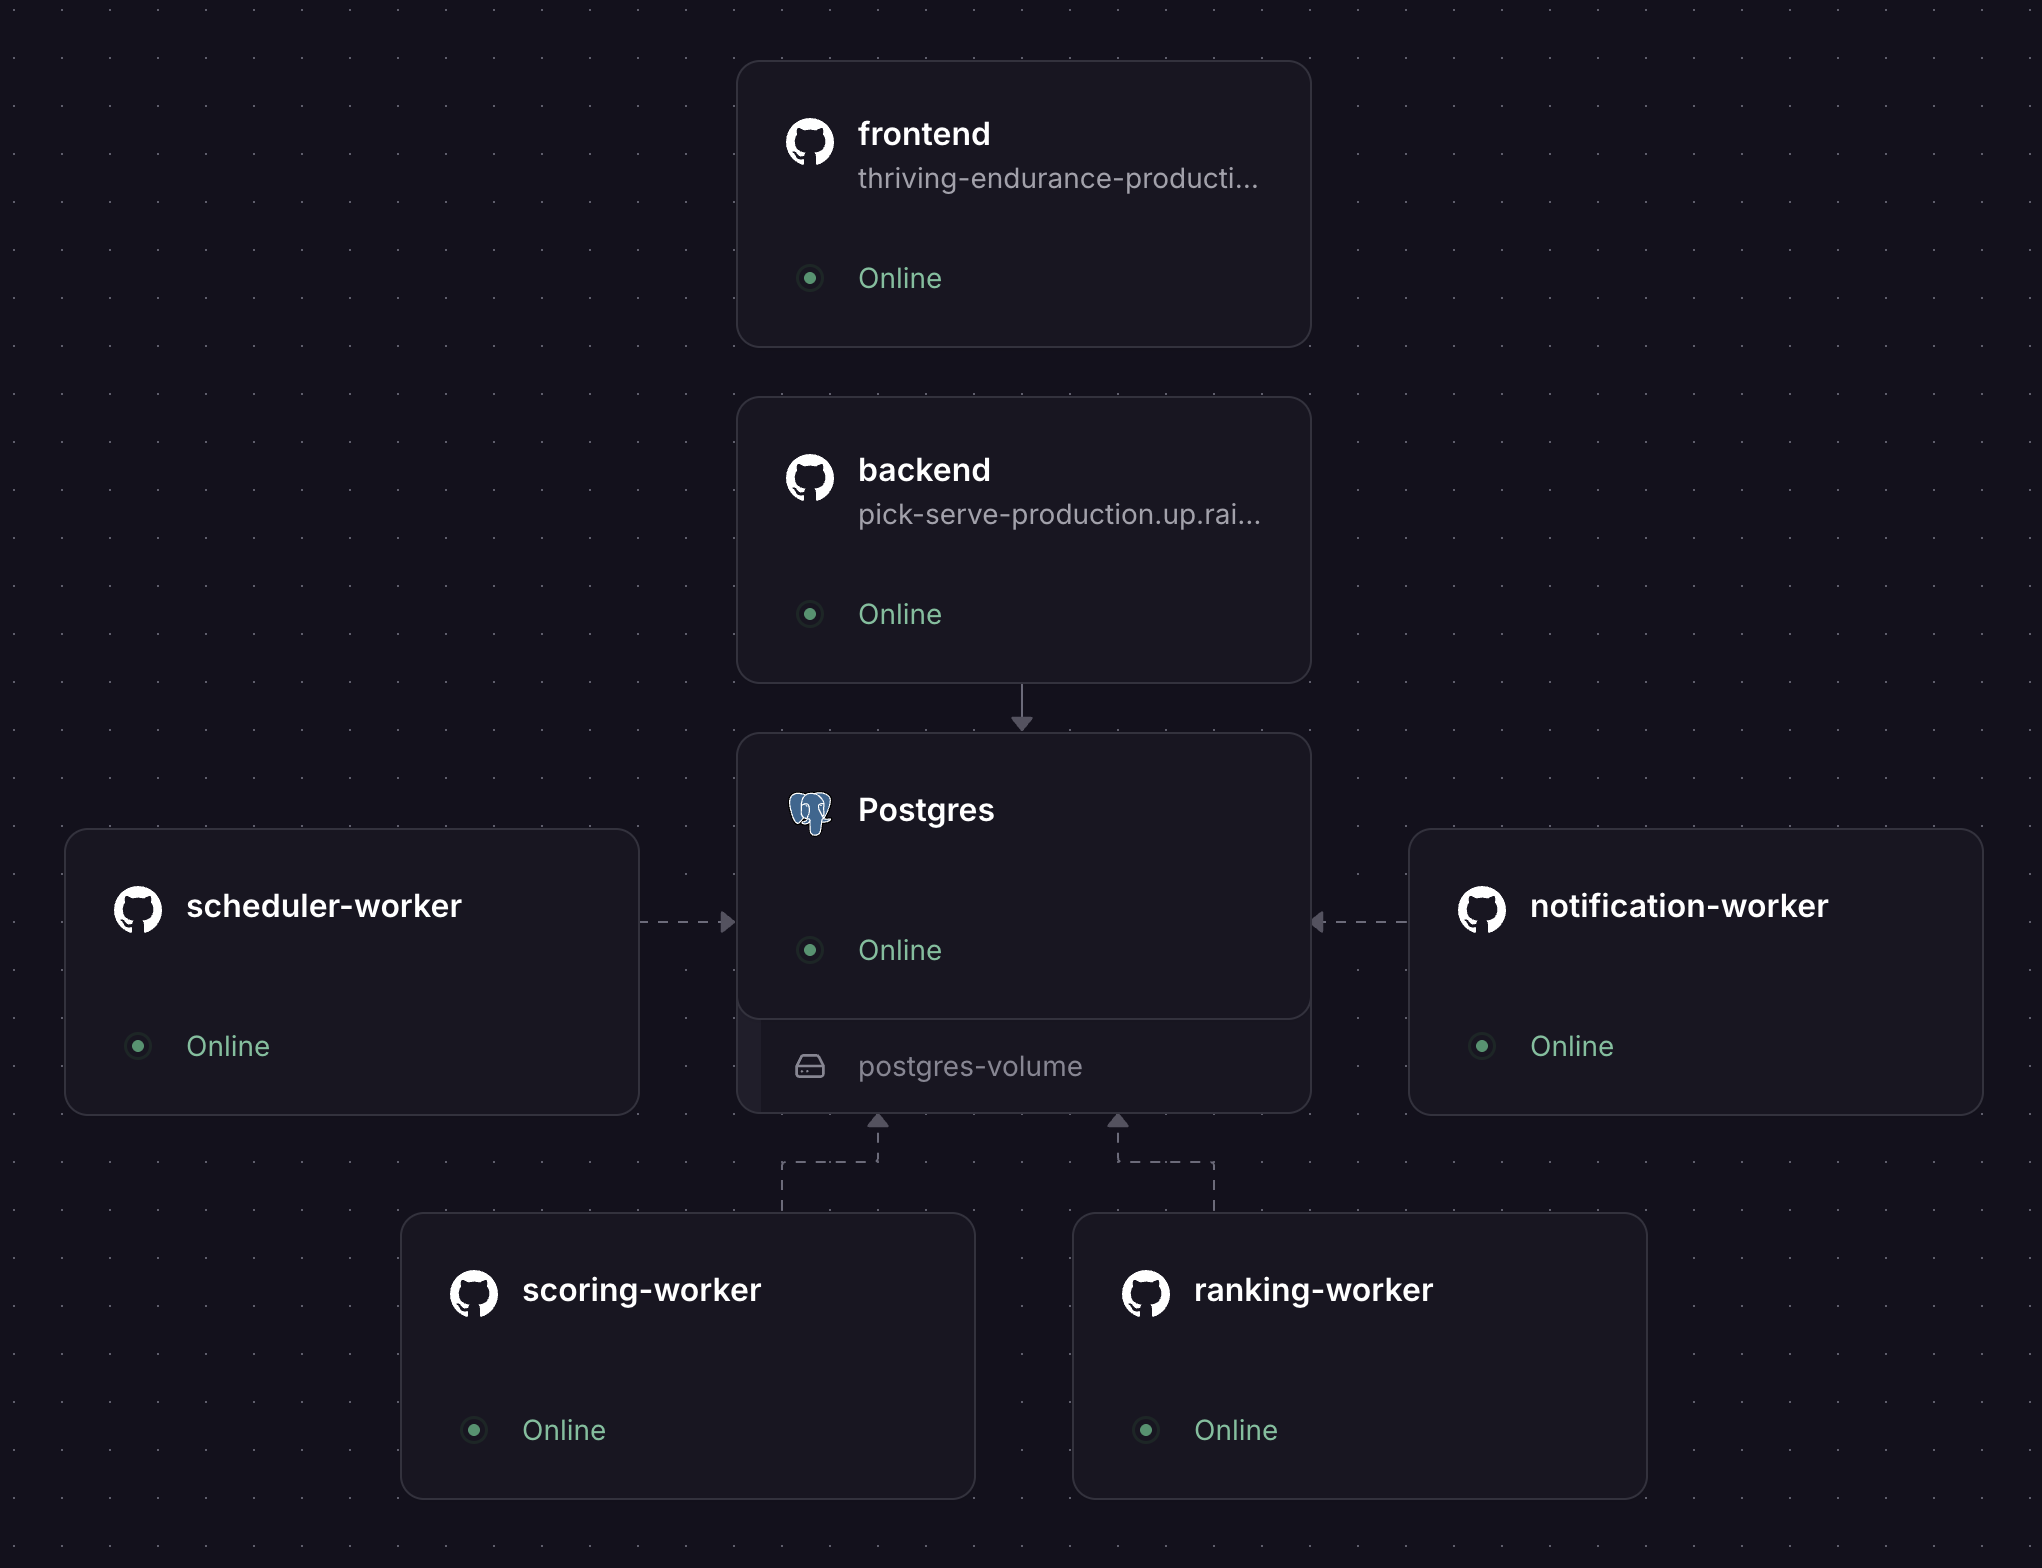
\includegraphics[width=\linewidth]{railway.png}
\caption{Dashboard de Railway con los seis servicios de Pick \& Serve activos: frontend, backend, scoring-worker, notification-worker, ranking-worker y scheduler. La base de datos corre como addon PostgreSQL de Railway y el broker como instancia CloudAMQP.}
\label{fig:railway}
\end{figure}

\begin{figure}[ht]
\centering
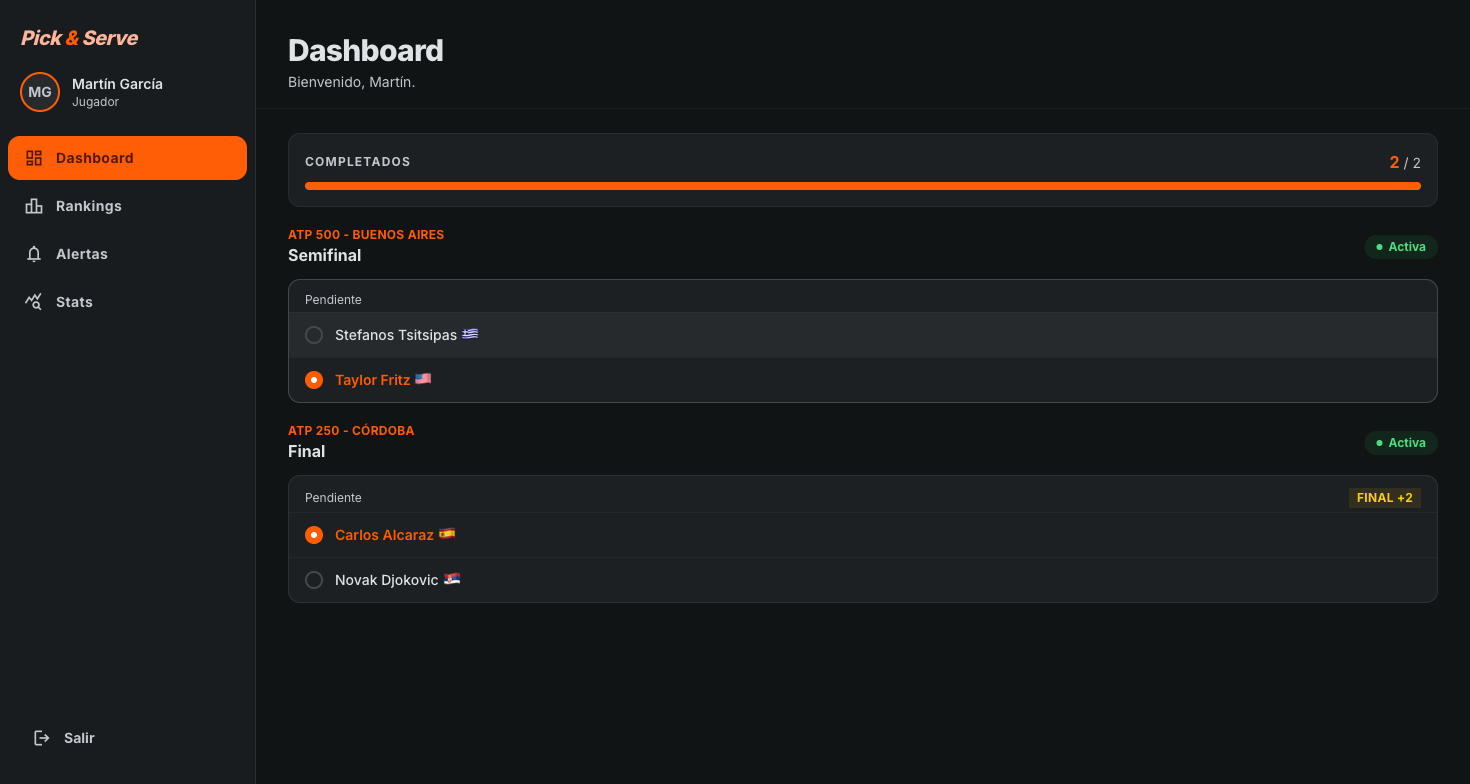
\includegraphics[width=0.88\linewidth]{screenshots/02_player_dashboard.png}
\caption{Dashboard del jugador Martín García con las jornadas abiertas y los partidos disponibles para pronosticar. El badge FINAL +2 indica el bonus de puntos para la final.}
\label{fig:player-dash}
\end{figure}

\begin{figure}[ht]
\centering
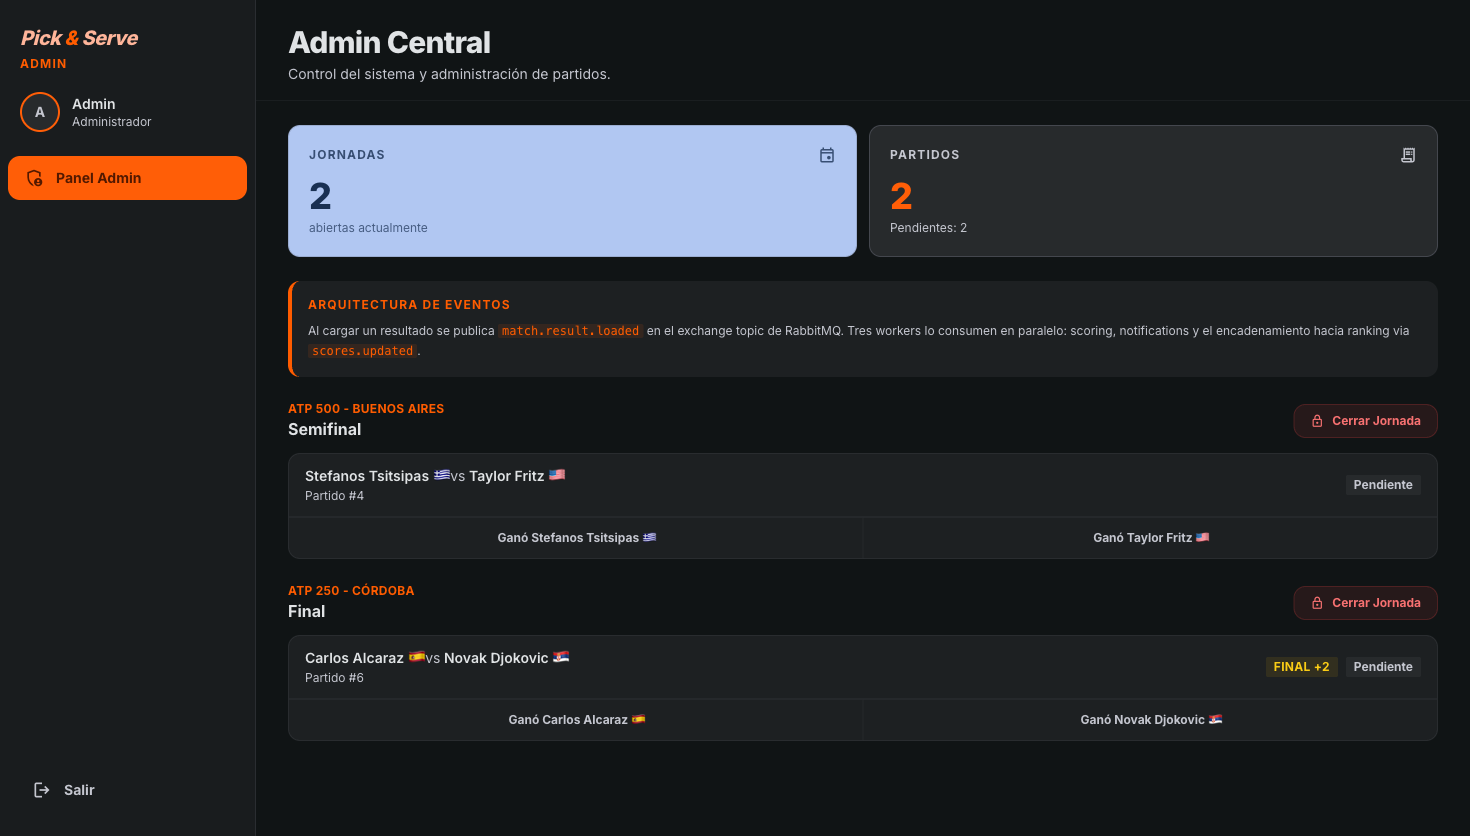
\includegraphics[width=0.88\linewidth]{screenshots/07_admin_dashboard.png}
\caption{Panel de administración con los partidos pendientes de resultado. La interfaz describe en línea el flujo de eventos: al cargar un resultado se publica \code{match.result.loaded} en el exchange topic y los workers lo consumen en paralelo.}
\label{fig:admin-panel}
\end{figure}

\begin{figure}[ht]
\centering
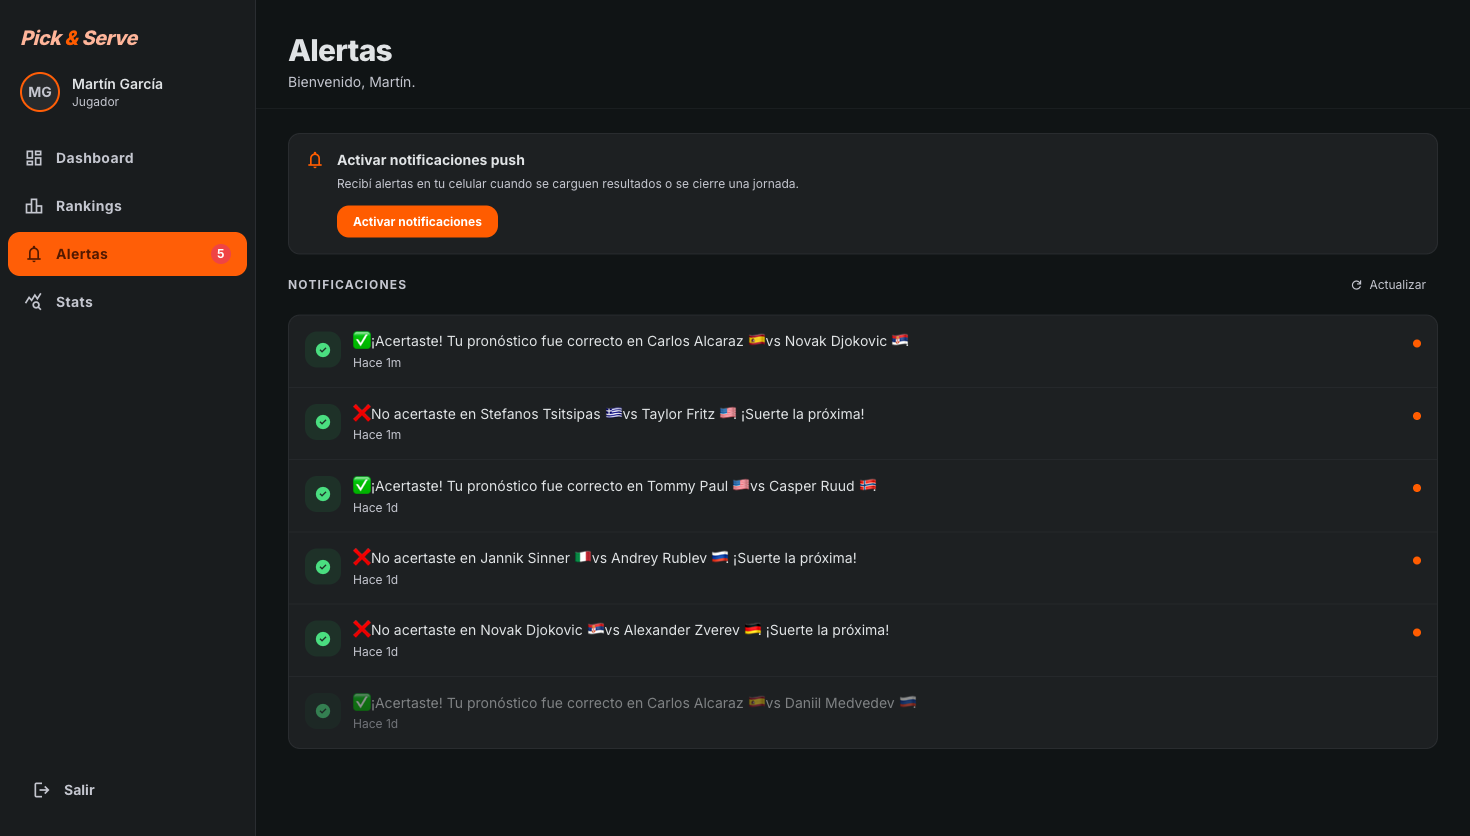
\includegraphics[width=0.88\linewidth]{screenshots/12_player_notifications_after_results.png}
\caption{Alertas del jugador tras cargar los resultados. Las dos notificaciones marcadas ``Hace 1m'' corresponden exactamente a los dos resultados que el administrador acaba de ingresar: el Notification Worker las generó de forma asíncrona al procesar \code{match.result.loaded}, sin bloquear la respuesta de la API.}
\label{fig:notif}
\end{figure}

\begin{figure}[ht]
\centering
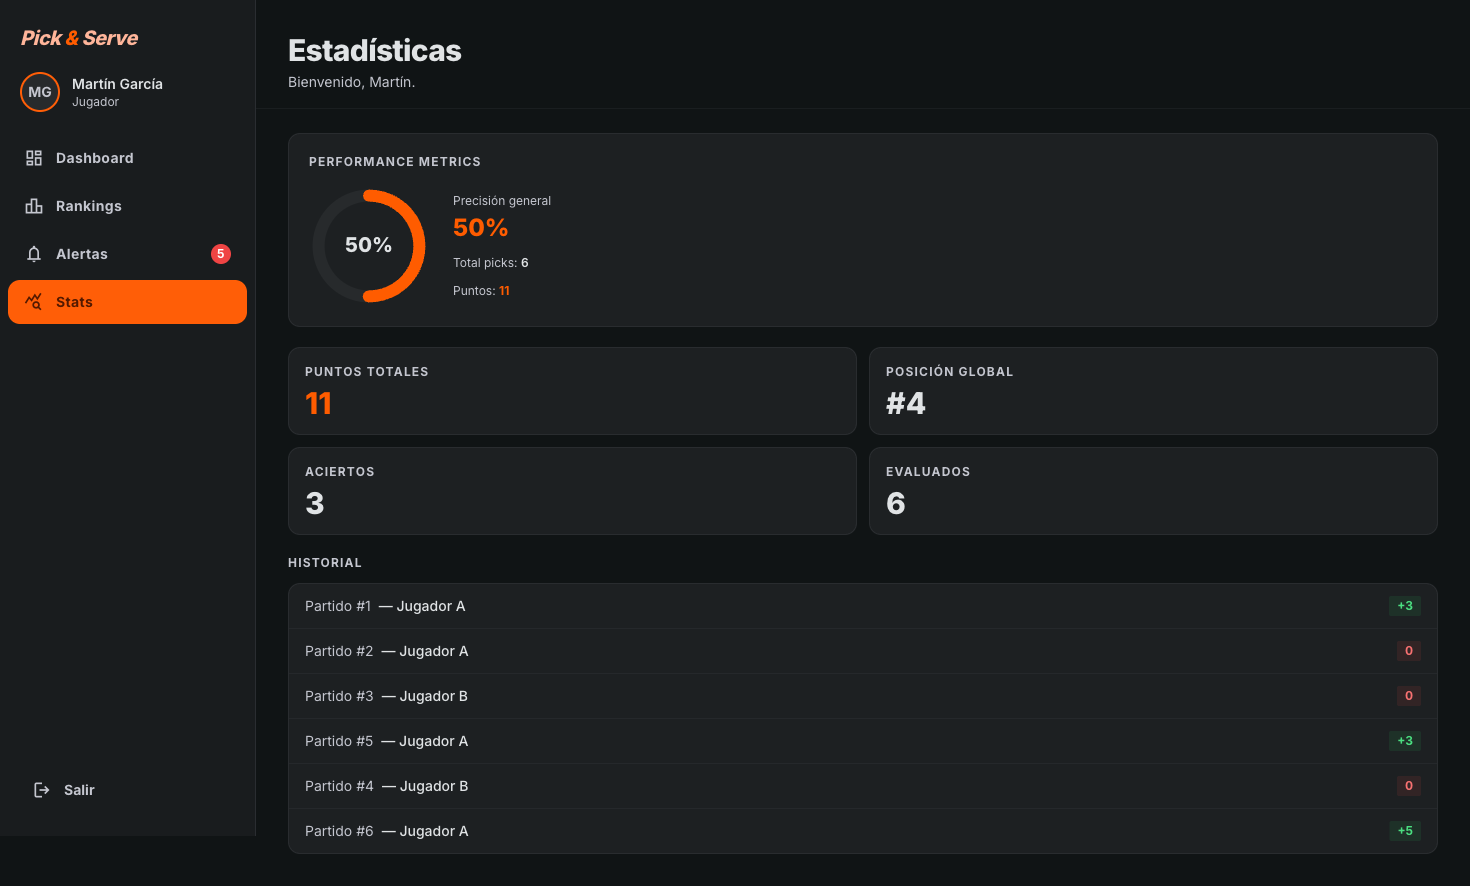
\includegraphics[width=0.88\linewidth]{screenshots/13_player_stats_after_results.png}
\caption{Estadísticas del jugador tras el cierre de la jornada. El Partido \#6 (la final) muestra +5 puntos: el Scoring Worker aplicó el acierto base (+3) y el bonus de final (+2) sin intervención manual.}
\label{fig:stats}
\end{figure}

\begin{figure}[ht]
\centering
\begin{minipage}{0.47\linewidth}
  \centering
  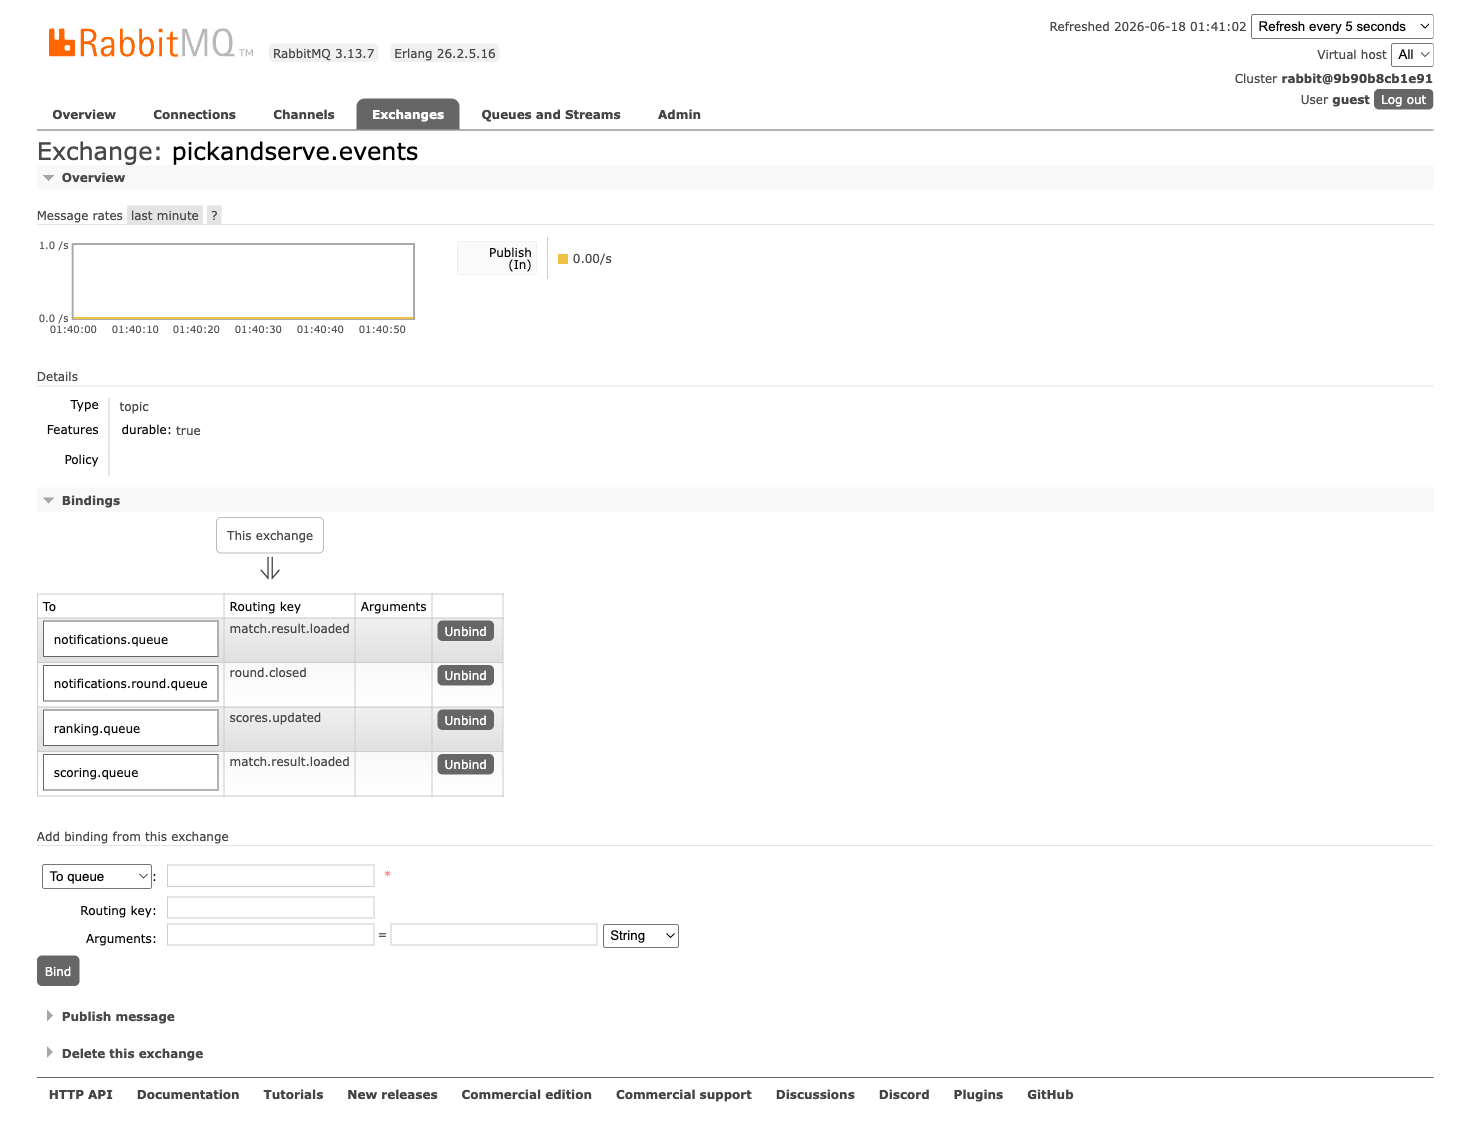
\includegraphics[width=\linewidth]{screenshots/rabbitmq_exchange_bindings.png}
\end{minipage}\hfill
\begin{minipage}{0.47\linewidth}
  \centering
  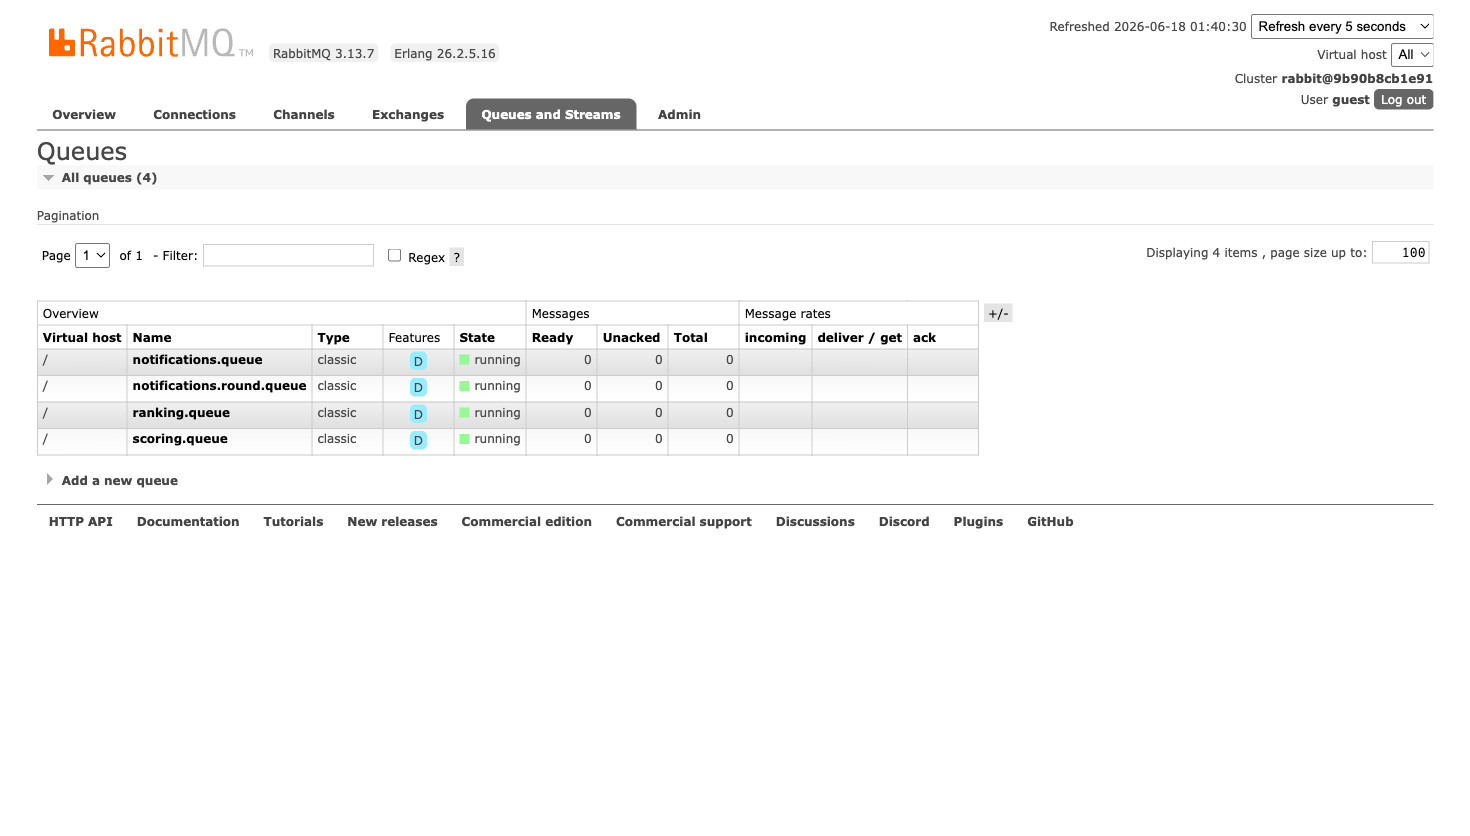
\includegraphics[width=\linewidth]{screenshots/rabbitmq_queues.png}
\end{minipage}
\caption{Consola de administración de RabbitMQ. Izquierda: exchange \code{pickandserve.events} de tipo topic con sus cuatro bindings: \code{scoring.queue} y \code{notifications.queue} suscritas a \code{match.result.loaded}, \code{ranking.queue} a \code{scores.updated}, y \code{notifications.round.queue} a \code{round.closed}. Derecha: las cuatro colas en estado \code{running} con persistencia durable activada (flag D).}
\label{fig:rabbitmq}
\end{figure}

\begin{figure}[ht]
\centering
\begin{minipage}{0.28\linewidth}
  \centering
  \includegraphics[width=\linewidth]{screenshots/notificacion_acierto.PNG}
\end{minipage}\hspace{3cm}
\begin{minipage}{0.28\linewidth}
  \centering
  \includegraphics[width=\linewidth]{screenshots/notificacion_no_acierto.PNG}
\end{minipage}
\caption{Notificaciones push recibidas en el dispositivo móvil. El Notification Worker entrega un aviso personalizado por cada pronóstico evaluado a través de la API Web Push, tanto en caso de acierto como de fallo.}
\label{fig:push}
\end{figure}
